\documentclass[conference]{IEEEtran}
%\IEEEoverridecommandlockouts
% The preceding line is only needed to identify funding in the first footnote. If that is unneeded, please comment it out.
\usepackage{cite}
\usepackage{amsmath,amssymb,amsfonts}
\usepackage{algorithmic}
\usepackage{graphicx}
\usepackage{textcomp}
\usepackage{url}
\usepackage{xcolor}
\def\BibTeX{{\rm B\kern-.05em{\sc i\kern-.025em b}\kern-.08em
    T\kern-.1667em\lower.7ex\hbox{E}\kern-.125emX}}
    
    
\setcounter{secnumdepth}{5}
\setcounter{tocdepth}{5}

\makeatletter
\newcommand\subsubsubsection{\@startsection{paragraph}{4}{\z@}{-2.5ex\@plus -1ex \@minus -.25ex}{1.25ex \@plus .25ex}{\normalfont\normalsize\bfseries}}
\newcommand\subsubsubsubsection{\@startsection{subparagraph}{5}{\z@}{-2.5ex\@plus -1ex \@minus -.25ex}{1.25ex \@plus .25ex}{\normalfont\normalsize\bfseries}}
\makeatother

\newcommand{\ulsi}[1]{\!\overline{\,{#1}}} % underline short italic
\newcommand{\uls}[1]{\mskip.5\thinmuskip\underline{\mskip-.5\thinmuskip {#1} \mskip-.5\thinmuskip}\mskip.5\thinmuskip} % underline short
   
\begin{document}

\title{Linear Regression: Deep Learning}

\author{\IEEEauthorblockN{Olaniyi Bayonle Alao}
\IEEEauthorblockA{\textit{Summer Term, 2021} \\
\textit{Bachelor of Electronic Engineering} \\
\textit{Hochschule Hamm-Lippstadt}\\
Lippstadt, Germany \\
olaniyi-bayonle.alao@stud.hshl.de}
}

\maketitle

\begin{abstract}
talk about the data example prediction that will/was done using sck-kit.  Then talk about what linear regression, why it is used......... 

this paper talks about linear regression in the context of deep learning. Linear regrression is a statictical term that uses a dependent and independent variable to make predictions. in these paper, the use case of linear regression is used to predict data in machine learning. The data were gotten from kaggle.com. the data is a data of the titanic survivers and the model was trained using sci-kit or tensor flow.

data cleasing was done using pandas a python library to prepare the data for model training.

regression analysis as a whole is a stastical method used to understand the relation between dependent and independent variables.


with the rise in the amount of data we have access to and increase in the performance of computers, Machine Learning a subset of Artificial inteligence has seen a significant growth. machine learning refers to  is the ability of applications to get better at doing things without necessarily a change in the code base them is something that has really been helpful. 

even though machine learning isn't a new concept, it is fast gaining recognization and changing lives thanks to the increase in the processing power of computers over the years to be able to process big data at a level that has never been experienced.


\end{abstract}
\begin{IEEEkeywords}
machine learning, linear regression, deep learning, sci-kit
\end{IEEEkeywords}
Unless otherwise stated, the main reference for facts, mathematical models and terminologies used in this research paper is gotten from \cite{massaron2016regression}
\section{Diagrams}
Include diagram for machine learning automatically adapting to change?? get idea from fig 1-3 page 25 of [hands-on machine learning with scikit-learn]
\section{Introduction}
Due to an explosive increase in the amount of data generated from different internet connected devices -Cyber-Physical-Systems (CPS)-, there has been an increase in the need to make sense of this "big data" to ensure the proper and productive functioning of businesses. By 2026, the data generation from global air fleet is projected to reach 98 billion gigabytes \cite{oliver_wyman}. Thanks to the recent advancements in the information processing capabilities of computers, making sense of this huge chunk of data is now possible using data analysis techniques and Machine learning to clean and make prediction from this datasets. Machine learning is the ability of machine -software application- to learn and make predictions without being programmed to do so. They are able to learn and get better with an increase in the amount of data they are being fed through through their grounded mathemical foundations.

\quad Linear regression is a statistical test used to find out the relationship between independent and dependent variables in a data set using mathematical formular. They can also be used in projecting new relationship between the dependent and independent variables that has not been discovered.
Even though linear models - linear regression - are quite simple to develop and understand, as well as good at predicting linear relationships, their approximation of nonlinear relationships have been found to be mostly unsatisfactory \cite{article_lee}. This paper goes more into the mathematical details 
this paper gives a profound, yet understandable mathematical description of Linear regression, relevant parts of the framework -Sci-Kit- used to perform predictions on the example dataset in the context of Machine learning using the Python programming language.

\section{Theoretical Background}
\subsection{Machine Learning}
According to \cite{ibm_cloud_education_2020}, "Machine learning is a branch of artificial intelligence (AI) focused on building applications that learn from data and improve their accuracy over time without being programmed to do so". Examples of applications built using machine learning trained models are email filters with the ability to distinguish between desired emails and spams, auto-suggestion/auto-correct in many typing applications, self-driving vehicles, amongst others. Machine learning techniques have the advantage of automatically adapting to change detected in trends from data. Likewise, they help reduce the complexity in writing application that are somethings difficulty or even impossible to implement using traditional algorithms. Methods used in training a Machine learning model can be grouped into three main categories.

	\begin{itemize}
		\item Supervised Learning
		
		This is a type of machine learning technique in which the algorithm is fed with an input and output dataset of desired solution. The desired output data is otherwise known as lables. These information help train the machine lerning model in the precise prediction of output when given a related output after being trained. Some examples of common algotithms used for supervised learnings are regression analysis - linear regression, etc.-, decision trees, amongst others.\cite{theobald2017machine} The two types of supervised learning techniques used are classification and regression.
		\item Unsupervised Learning
		
		This refers to the machine learning technique in which the algorithm is only fed with input data for the training process. The model learns "unsupervised" by finding out and grouping patterns in inputted datasets. Unlike supervised learning, they require large amount of unlabeled datasets to train -properly find patterns in datasets.
		\item Semisupervised Learning
		
		this is a learning technique that uses both labeled -input and desired output- and unlabled -only input- datasets for training machine lerning models.
	\end{itemize}
The other methods used in training a machine learning model are reinforcement learning and deep learning. Deep learning is a subset of machine learning who's algorithm defines an artificial neural network -ANN- that is designed to emulate the way an human brain learns, and unsupervised or semisupervised learning technique to train \cite{ibm_cloud_education_2020}. On other hand, reinforcement learning is a reward based learning in the sense that the machine leaning is trained by being given a point for reaction to certain events.

\subsection{Linear Regression Model}
Regression 
is a predictive analysis with a long but glorious history from its successful applications to problems in the statistics and economics domain. Regression is a kind of supervised learning technique for determining the best fit line to describe patterns in data: linear regression uses a straight line to describe these patterns.\cite{theobald2017machine}. The best fit line is the line that reduces the summed squared difference between the value of the line of a certain value \textbf{\textit{x}} and its corresponding \textbf{\textit{y}} values \cite{from main reference}. The mathematical expression for linear regression is:
	\begin{equation}
		y = \beta\label{beta}X + \beta\textsubscript{0}
	\end{equation}
	Where y is the dependent variable, X is the independent variable of the equation, $\beta$ is a cofficient which reperesnts the slope of the regression line, $\beta$\textsubscript{0} is a constant value called the \textbf{bias}. Equation \eqref{beta} is the same as the equation of a straight line in linear algebra.
	
	The independent variable X in \eqref{beta} is calculated using the mathematical expression below:
	\begin{equation}
    		%\frac{\sum{(x-x)(y-y)}{6}
		X = \frac{\sum{}(x-\overline{x})(y-\overline{y})}{\sum{}(x-\overline{x})^2}
		%\sum{}\frac{(x-x)}{5}
	\end{equation}	
	Where $\overline{x}$ and $\overline{y}$ are the mean values of all the respective x and y variables.
	
	
Linear regression analysis can be sub-divided into simple and multiple linear regression depending on the number of their independent variables. If the independent variable is one, the regression is said to be a simple linear regression, but if the independent variable is more than one, it is a multiple linear regression. In this paper, we will make analysis using the simple linear regression model.

\subsection{Model Evaluation}
The prediction made by the model using equation \eqref{beta} can be evaluated using the statistical methods below to find out how close the predicted value is to the the actual value.
\subsubsection{R\textsuperscript{2}}
this is otherwise known as the coefficient of determination or the coefficient of multiple determination is a measure of how close the best fit line is to the original data using a simple mean. The value of the output of this calculation ranges from 0 to 1\cite{DAE79009}. A value of 1 refers to the fact that all the points fits 100$\%$ to the the regression line. The lesser the value, the farther the points are to the regression line. The coefficient of determination is defined by the following equation:

	\begin{equation}
    		%\frac{\sum{(x-x)(y-y)}{6}
		R\textsuperscript{2} = \label{three}\frac{\sum_{i=1}^{n}(\hat{y_i}-\overline{y})^2}{\sum_{i=1}^{n}(y_i-\overline{y})^2}
		%\sum{}\frac{(x-x)}{5}
	\end{equation}
	
	Where n is the number of observations i.e. total number of variables, $\hat{y_i}$ is the estimated value of the dependent variable for the i\textsuperscript{th} observation computed by the regression equation, $y_i$ is the observed value of the dependent variable for the i\textsuperscript{th} observation and $\overline{y}$ is the mean of all n observations of the dependent variable \cite{DAE79009}

\subsubsection{Mean Squared Error}
Mean Squared Error (MSE) is a performance measure that helps determine how much error is made in the predicted value in relation to the the actual value of the ouput given the same input. The equation of the calculation is denoted by:

	\begin{equation}
    		%\frac{\sum{(x-x)(y-y)}{6}
		MSE = \label{four}\frac{1}{n}\sum_{i=1}^{n}(y_i-\hat{f}(x_i))^2
		%\sum{}\frac{(x-x)}{5}
	\end{equation}
	where $x_i$ is a vector of all i\textsuperscript{ith} observation, $\hat{f}$ is the prediction function. The lower the value of MSE, the more accurate the prediction is.
\section{Algorithm Implementation}
All the algorithm needed  for prediction using the linear regression model have been implemented in machine learning libraries like Scikit learn which we will be using in this paper.
\subsection{Libraries and Tools used}
\subsubsection{Scikit Learn}
Scikit learn is an open-source python library that provides algorithms that are used in machine learning. This library provide functionalities for solving machine learning jobs like 
regression, classification, clustering, model selection, pre-processing - like spliting data sets into test and train subsets -amongst others \cite{scikit_learn}. The scikit-learn API are designed around this main design principles which are consistency - all objects (basic or composite) share a consistent interface composed of a limited set of methods -, inspection - parameters are exposed as public attributes -, composition, sensible defaults - provides understandable default parameters which gives baseline solution for tasks at hand -and nonproliferation of classes - datasets are represented as NumPy arrays or SciPy sparse matrices \cite{sklearn_api}.
\subsubsection{Numpy}
NumPy is an open-source Python library that that provides routines that allows for fast operations on multidimensional arrays, including mathematical, logical, shape manipulation, sorting, selecting, I/O, discrete Fourier transforms, basic linear algebra, basic statistical operations, random simulation\footnote{https://numpy.org/doc/stable/user/whatisnumpy.html}.
\subsubsection{Pandas}
Pandas is an open-source data analysis and manipulation python library that allows high-performance easy exploration, cleaning and processing of tabular data structures in Python\footnote{https://pandas.pydata.org/docs/}.
\subsubsection{Matplotlib}
Matplotlib is a Python library used along with Numpy for creating static, animated and interactive visualization of data\footnote{https://matplotlib.org/}.
\subsubsection{Seaborn}
Seaborn is a Python library which builds upon the functionalities of matplotlib and integrates closely with pandas data structures for making statistical graphics to datasets\footnote{https://seaborn.pydata.org/introduction.html}.
\section{Practical Example}
In this paper, the california housing datasets from \cite{KELLEYPACE1997291} included in the scikit sklearn datasets library is used to predict train and prediction the average prices of housing in california using linear regression. 
\subsection{Preparing Data}
The dataset has 20,640 instance number, 8 numeric predictive atrributes and 1 target attribute which is expected output of the prediction, which is the median house value for California districts. A block group is the smallest geographical unit for which the U.S. Census Bureau publishes sample data (a block group typically has a population of 600 to 3,000 people), the datasets were obtained in a 1990 census \cite{KELLEYPACE1997291}.
The predictive attributes have the following information: 
	\begin{itemize}
		\item MedInc: represents the median income in a block.
		\item HouseAge: represents the median house age in block.
        		\item AveRooms: represents the average number of rooms.
        		\item AveBedrms: represents the average number of bedrooms.
        		\item Population: represents the population in the block.
        		\item AveOccup: represents the average house occupancy.
	        \item Latitude: represents the house block latitude.
        		\item Longitude: represents the house block longitude.
	\end{itemize}
	This dataset can download from scikit learn online sklearn.datasets repository by using the following code "from sklearn.datasets import $fetch\_california\_housing 
california = fetch\_california\_housing()$"


The data used in this example is gotten from sckit learn. this returns the following datasets with each attribute meaning....get from this link \url{https://scikit-learn.org/stable/modules/generated/sklearn.datasets.fetch_california_housing.html}.



	\begin{itemize}
		\item Figure \ref{fig:placeholder} shows the import statments for the functions and libraries that are used.the libraries were imported
		\item Figure \ref{fig:overview_dataset_with_target} shows the overview of the data as a  pandas dataframe which include the target feature column.
		\item Figure \ref{fig:pearson_correlation_of_the_dataset} shows a table of the pearson correlation of the attribes to each other using pandas library. The closer the value are to one, the more thery are related to each other. It can be seen from the figure that the median income in a block has the highest correlation to the target variable. Which is why we will be using it as the variable for training our model. This visualization can also be seen in the heatmap drawn with seaborn in figure \ref{fig:correlation_heatmap}.
		\item Figure \ref{fig:reshape_dataset} shows the code snipet that was used to transform the X variable to a 2d array as expected by scikit learn regression function. X variable is a 2d array respresenting the median income per block and the y variable is the target representing the median house value in unit of 100,000.
		\item Create an instance of the linear regression class which is used for training the model.
		\item Figure \ref{fig:coefficients_intercepts} shows the coefficients and intercepts of the equation for predicting variables calculated by the sklearn fit() method.
		\item Try out the prediction using the test dataset. Figure \ref{fig:predicted_vs_actual} shows the first ten predicted value and the actual value expected. There seems to be some offset in the predictions.
		\item Figure \ref{fig:r_mse_value} shows the $R^2$ and MSE value of the prediction. The value explains the reason why there were some offsets in the prediction. The model can be said to have underfitted the training data because the feature used did not provide enough information to make a good prediction as we understand that the house prices are influenced by many factors unlike just one variable that was used.
		\item Figure \ref{fig:predicted_vs_actual_graph} shows a plot of the regression line of first 30 predicted values to their actual target marked in red. It can be seen that some of the target value are quite far away to the regression line drawn.
		
\item Datasets were then split and randomized into 20 percent for training and testing the model.
\item the dataset was created as a panda data frame to allow easy manipulation I guess. then the target column was added to the dataset columns which will be the y variable
\item a description of the data was manage to get a quick statistics on the data being worked on.
\item the input variable is the AveRooms ............ it total-room, which the totatl number of rooms in a block,
\item We'll randomize the data, just to be sure not to get any pathological ordering effects that might harm the performance of Stochastic Gradient Descent.[google colab]
\item use the 
\end{itemize}

\subsection{Result and discussion}
From the result of the predictions, it can be seen that the model underfitted the training data and as a result was not able to make the right prediction of the target value. The MSE value was 0.45 which showed that there were significant errors in predicting the values.

\section{Conclusion}
finish by highlighting the strenth of linear regression as well as the shorcomings.

\newpage
\begin{figure}[htbp]
	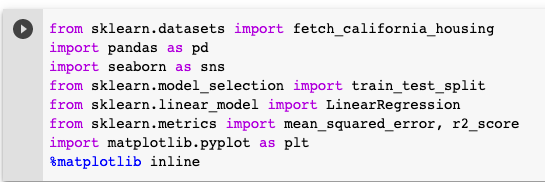
\includegraphics [scale=0.5]{figures/import_statements.png}
	\caption{Import statements}
	\label{fig:placeholder}
\end{figure}

\begin{figure}[htbp]
	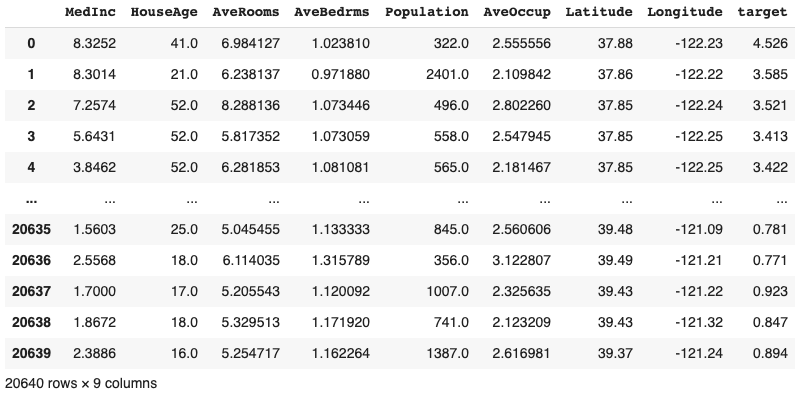
\includegraphics [scale=0.5]{figures/overview_dataset_with_target.png}
	\caption{Dataset overview including the target column}
	\label{fig:overview_dataset_with_target}
\end{figure}

\begin{figure}[htbp]
	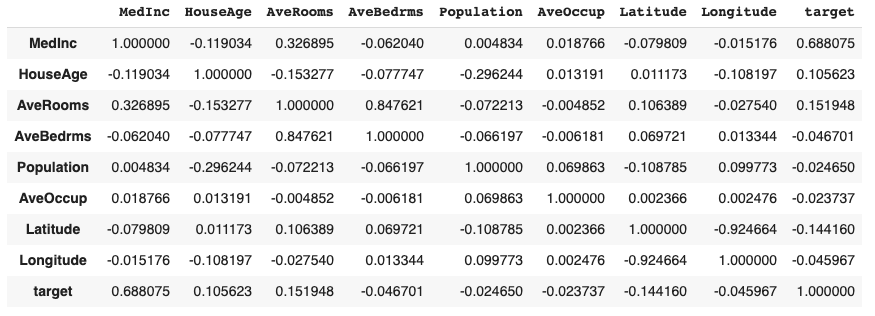
\includegraphics [scale=0.5]{figures/pearson_correlation_of_the_dataset.png}
	\caption{Pearson correlation of the dataset attributes}
	\label{fig:pearson_correlation_of_the_dataset}
\end{figure}

\newpage
\begin{figure}[htbp]
	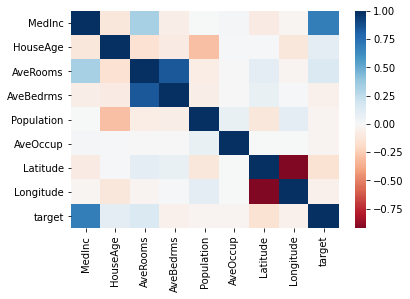
\includegraphics [scale=0.5]{figures/correlation_heatmap.png}
	\caption{Pearson correlation heatmap of the dataset attributes}
	\label{fig:correlation_heatmap}
\end{figure}

\begin{figure}[htbp]
	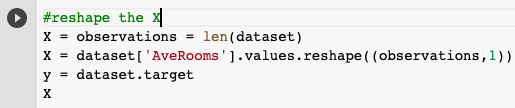
\includegraphics [scale=0.5]{figures/reshape_dataset.png}
	\caption{Code snippet for reshaping and extracting the X and y variable for the regression analysis}
	\label{fig:reshape_dataset}
\end{figure}

\begin{figure}[htbp]
	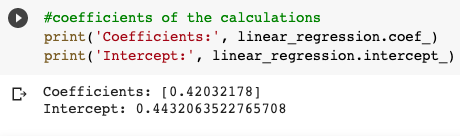
\includegraphics [scale=0.5]{figures/coefficients_intercepts.png}
	\caption{Coefficients and intercept of the equation as calculated by sklearn}
	\label{fig:coefficients_intercepts}
\end{figure}


\begin{figure}[htbp]
	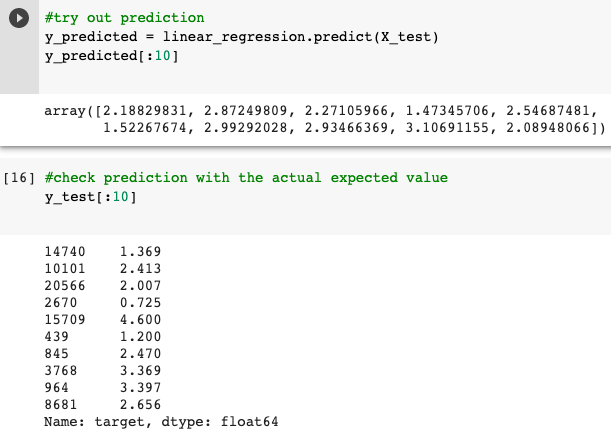
\includegraphics [scale=0.5]{figures/predicted_vs_actual.png}
	\caption{Predicted value vs actual value}
	\label{fig:predicted_vs_actual}
\end{figure}


\begin{figure}[htbp]
	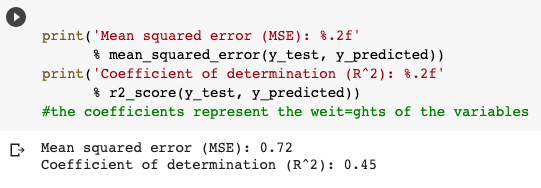
\includegraphics [scale=0.5]{figures/r_mse_value.png}
	\caption{$R^2$ and MSE value of the model}
	\label{fig:r_mse_value}
\end{figure}


\begin{figure}[htbp]
	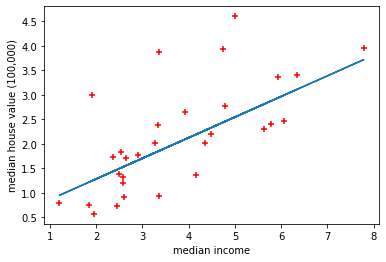
\includegraphics [scale=0.5]{figures/predicted_vs_actual_graph.png}
	\caption{Plot of the regression line to the actual target value}
	\label{fig:predicted_vs_actual_graph}
\end{figure}

\bibliographystyle{plain}
\bibliography{references}
\end{document}
